\chapter{Fundamentos teóricos}
\label{ch:fundamentos}

Este capítulo recoge los conceptos de mecánica orbital necesarios para seguir el resto del trabajo: la órbita y los parámetros que la describen, las perturbaciones que la apartan del caso ideal y las maniobras orbitales que la inteligencia artificial deberá aprender a ejecutar.

\section{El problema de los dos cuerpos y la órbita kepleriana}
\label{sec:dos-cuerpos}

El movimiento de un satélite alrededor de un cuerpo central de masa $M$ se describe, en primera aproximación, mediante el problema de los dos cuerpos: se desprecia todo salvo la atracción gravitatoria mutua (Figura~\ref{fig:dos-cuerpos}). La ecuación del movimiento relativo es:
\begin{equation}
  \ddot{\vec{r}} = -\frac{\mu}{r^{3}}\,\vec{r},
  \qquad \mu = G M,
  \label{eq:dos-cuerpos}
\end{equation}
donde $\vec{r}$ es el vector de posición del satélite respecto al centro y $\mu$ el parámetro gravitatorio del cuerpo. Esta ecuación no es más que la atracción gravitatoria mutua expresada como aceleración: al dividir la fuerza que el cuerpo central ejerce sobre el satélite, $F = G\,M\,m/r^{2}$, entre la masa de este se obtiene una aceleración de módulo $\mu/r^{2}$ dirigida hacia el centro, que es precisamente lo que recoge la Ecuación~\eqref{eq:dos-cuerpos}. Cada cuerpo atrae al otro con una fuerza de igual módulo y sentido opuesto (ley de gravitación de Newton), dirigida a lo largo de la recta que los une; $\vec{r}$ es el vector de posición
 del satélite respecto al cuerpo central y $r$ su módulo. 

\begin{figure}[htbp]
  \centering
  
\includegraphics[width=0.85\textwidth]{tex/imagenes/fig_dos_cuerpos.pdf}
  \caption{Atracción gravitatoria mutua en el problema de los dos cuerpos. Elaboración propia.}
  \label{fig:dos-cuerpos}
\end{figure}

La solución de la Ecuación \ref{eq:dos-cuerpos} es una cónica (círculo, elipse, hipérbola, parábola) con el cuerpo central en uno de sus focos (primera ley de Kepler). Para las órbitas ligadas ---las de interés aquí--- esa cónica es una elipse, cuyo tamaño y forma quedan fijados por el semieje mayor $a$ y la excentricidad $e$.

Dos relaciones fundamentales se usarán a lo largo del trabajo. La energía orbital específica depende solo del semieje según la Ecuación \ref{eq:energia-fund}:

\begin{equation}
  \varepsilon = -\frac{\mu}{2a},
  \label{eq:energia-fund}
\end{equation}
de modo que reducir la energía (por ejemplo, con el arrastre) reduce $a$ y, por tanto, la altitud. La ecuación de la \textit{vis-viva} da la velocidad en cualquier punto de la órbita (Ecuación \ref{eq:vis-viva}):
\begin{equation}
  v^{2} = \mu\left(\frac{2}{r} - \frac{1}{a}\right).
  \label{eq:vis-viva}
\end{equation}
Por último, el periodo orbital (tercera ley de Kepler) es (Ecuación \ref{eq:periodo}):
\begin{equation}
  T = 2\pi\sqrt{\frac{a^{3}}{\mu}}.
  \label{eq:periodo}
\end{equation}

El semieje y la excentricidad fijan el tamaño y la forma de la elipse, pero no cómo está orientada en el espacio ni dónde se encuentra el satélite sobre ella. Describir una órbita por completo exige, por tanto, un conjunto más amplio de parámetros ---los elementos orbitales clásicos---, que se presentan en el apartado siguiente.

\section{Los elementos orbitales clásicos}
\label{sec:elementos}

Una órbita kepleriana queda completamente determinada por seis parámetros, los elementos orbitales clásicos, que se pueden observar en la Figura~\ref{fig:elementos}, que separan tres aspectos independientes: el tamaño y la forma de la elipse, la orientación de su plano y la posición del satélite.

\begin{itemize}
  \item \textbf{Tamaño y forma:}
    \begin{itemize}
      \item \textbf{Semieje mayor $a$} --- el tamaño de la órbita (y su energía).
      \item \textbf{Excentricidad $e$} --- cuánto se aparta de la circular.
    \end{itemize}
  \item \textbf{Orientación del plano:}
    \begin{itemize}
      \item \textbf{Inclinación $i$} --- ángulo del plano orbital respecto al plano de referencia (el ecuatorial del cuerpo).
      \item \textbf{Longitud del nodo ascendente $\Omega$ (\gls{RAAN})} --- el ángulo, medido en el plano de referencia desde una dirección fija (el punto Aries)\footnote{Dirección de referencia fija en el espacio: apunta al punto donde el Sol cruza el ecuador celeste en el equinoccio de primavera, y sirve de origen para medir ángulos como la ascensión recta $\Omega$.}, que localiza el nodo ascendente: el punto donde la
            órbita cruza dicho plano de sur a norte.
    \end{itemize}
  \item \textbf{Orientación de la elipse y posición:}
    \begin{itemize}
      \item \textbf{Argumento del perigeo $\omega$} --- orienta la elipse dentro de su plano (dónde está el punto más cercano).
      \item \textbf{Anomalía verdadera $\nu$} --- la posición del satélite sobre la órbita en un instante dado (el único que cambia con el tiempo en el caso
            kepleriano).
    \end{itemize}
\end{itemize}

Además de eso se muestra también la dirección de referencia, que siempre apunta hacia el punto de Aries.

\begin{figure}[htbp]
  \centering
  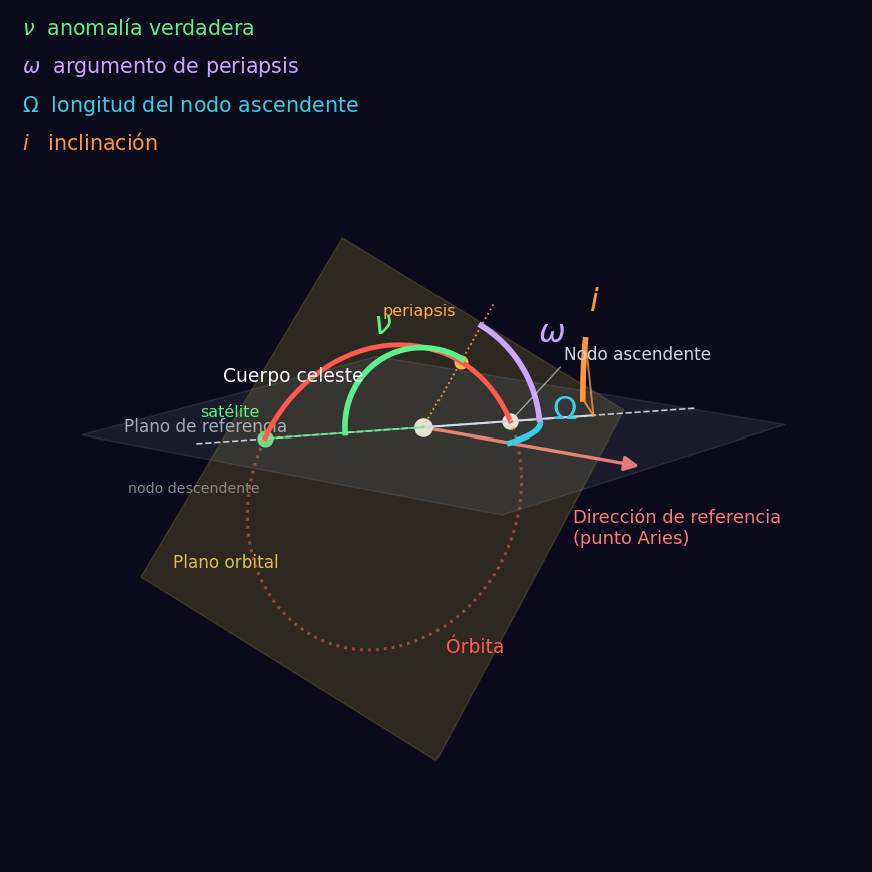
\includegraphics[width=0.9\textwidth]{tex/imagenes/fig_elementos_orbitales.png}
  \caption{Los seis elementos orbitales clásicos. Elaboración propia.}
  \label{fig:elementos}
\end{figure}

Bajo perturbaciones, estos elementos dejan de ser constantes: se habla entonces de elementos osculadores, que son los de la elipse kepleriana que en cada instante ajusta a la posición y velocidad reales. Su evolución es la que permite estudiar fenómenos como la regresión nodal (Capítulo~\ref{ch:desarrollo}).

Descrita ya la órbita en su forma, su orientación y su evolución, el paso natural es ver cómo se clasifican en la práctica según su altitud, lo que da lugar a los distintos regímenes orbitales.

\section{Regímenes orbitales}
\label{sec:regimenes}

Según su altitud, las órbitas terrestres se agrupan en varios regímenes de uso común (Figura~\ref{fig:regimenes}), que se nombrarán más adelante al plantear las maniobras de la \gls{IA}:
\begin{itemize}
  \item \textbf{\acrfull{LEO}} (órbita baja): altitudes comprendidas aproximadamente entre 200 y 2000~km. Es la región de la \gls{ISS} y de la mayoría de satélites de observación, y aquella en la que el arrastre atmosférico resulta relevante.
  \item \textbf{\acrfull{MEO}} (órbita media): entre los 2000~km y la altitud geoestacionaria. Alberga las constelaciones de navegación (\gls{GPS}, Galileo).
  \item \textbf{\acrfull{GEO}} (órbita geoestacionaria): a unos 35\,786~km de altitud, donde el periodo orbital coincide con el día sidéreo\footnote{Tiempo que tarda la Tierra en dar una vuelta completa respecto a las estrellas (unas 23~h 56~min), algo menor que el día solar de 24~h.} y el satélite aparenta permanecer fijo sobre un punto del ecuador. Es el destino típico de los satélites de telecomunicaciones.
\end{itemize}
El primer hito de la \gls{IA} del proyecto será, precisamente, una transferencia de Hohmann de \gls{LEO} a \gls{GEO} (Sección~\ref{sec:hohmann}).

\begin{figure}[htbp]
  \centering
  
\includegraphics[width=0.72\textwidth]{tex/imagenes/fig_regimenes_orbitales.pdf}
  \caption{Regímenes orbitales terrestres (\gls{LEO}, \gls{MEO} y \gls{GEO}) representados a escala. Elaboración propia.}
  \label{fig:regimenes}
\end{figure}

En todo lo anterior la órbita se ha tratado como una elipse ideal e inalterable. En la realidad, en cambio, diversas fuerzas la apartan de ese comportamiento perfecto: son las perturbaciones orbitales, que se examinan a continuación.

\section{Perturbaciones orbitales}
\label{sec:perturbaciones}

En la realidad, ninguna órbita es una elipse perfecta e inmutable: existen fuerzas adicionales, las perturbaciones, que la modifican. Las principales en un entorno planetario son:

\begin{itemize}
  \item \textbf{Achatamiento del planeta ($J_2$)}: el cuerpo central no es una esfera perfecta, lo que perturba el campo gravitatorio. Es una perturbación conservativa: no disipa energía, sino que hace precesar la órbita (Se explicará con más detalle más adelante).
  \item \textbf{Arrastre atmosférico (\textit{drag})}: la fricción con la atmósfera. Es disipativa: extrae energía y hace decaer la órbita hasta la reentrada.
  \item \textbf{Tercer cuerpo} (Sol, lunas) y \textbf{presión de radiación solar}, relevantes sobre todo en órbitas altas.
\end{itemize}

Para el alcance de este trabajo, las dos perturbaciones dominantes son $J_2$ y el arrastre; el resto se desprecia. El modelado e  implementación detallados de ambas se desarrollan en el  Capítulo~\ref{ch:desarrollo}.

Si las perturbaciones alteran la órbita de forma inevitable, las maniobras la modifican de manera deliberada y controlada; a estas últimas se dedica el apartado que cierra el capítulo.

\section{Maniobras orbitales}
\label{sec:maniobras}

Una maniobra cambia la órbita mediante el empuje de los motores. Su coste se mide por el $\Delta v$ (incremento de velocidad requerido), directamente ligado al consumo de combustible. El objetivo de la \gls{IA} del proyecto será ejecutar maniobras minimizando ese $\Delta v$.

\subsection{Transferencia de Hohmann}
\label{sec:hohmann}

La transferencia de Hohmann lleva un satélite entre dos órbitas circulares coplanarias (radios $r_1$ y $r_2$) mediante dos impulsos tangenciales, a través de una elipse de transferencia con semieje $a_t = (r_1+r_2)/2$. Es la transferencia de mínimo $\Delta v$ para ese cambio de radio, lo que la convierte en el caso de referencia ideal para validar al agente. Los impulsos vienen dados por las Ecuaciones \ref{eq:hohmann-dv1} y \ref{eq:hohmann}:
\begin{align}
  \Delta v_1 &= \sqrt{\frac{\mu}{r_1}}\left(\sqrt{\frac{2 r_2}{r_1+r_2}} - 1\right),
  \label{eq:hohmann-dv1}\\
  \Delta v_2 &= \sqrt{\frac{\mu}{r_2}}\left(1 - \sqrt{\frac{2 r_1}{r_1+r_2}}\right),
  \label{eq:hohmann}
\end{align}
y el coste total es $\Delta v_{\text{tot}} = \Delta v_1 + \Delta v_2$. El tiempo de transferencia es medio periodo de la elipse (Ecuación \ref{eq:hohmann-tiempo}):
\begin{equation}
  t_{\text{transf}} = \pi\sqrt{\frac{a_t^{3}}{\mu}}.
  \label{eq:hohmann-tiempo}
\end{equation}

\subsection{Cambio de plano}
\label{sec:cambio-plano}

Las maniobras anteriores modifican el tamaño de la órbita, pero no su orientación. Para cambiar el plano orbital ---por ejemplo, su inclinación $i$--- hay que girar el vector velocidad sin alterar (idealmente) su módulo. Un cambio puro de plano de ángulo $\Delta i$ sobre una órbita de velocidad $v$ cuesta (Ecuación \ref{eq:cambio-plano-fund}):
\begin{equation}
  \Delta v = 2\,v\,\sin\frac{\Delta i}{2}.
  \label{eq:cambio-plano-fund}
\end{equation}
El coste es proporcional a la velocidad: cambiar de plano resulta mucho más barato donde el satélite se mueve despacio, es decir, en el apogeo. Por eso, en una transferencia entre órbitas de distinto radio e inclinación, lo óptimo no es girar y transferir por separado, sino combinar ambas cosas repartiendo el giro entre los dos impulsos, con la mayor parte en el de mayor altura (menor velocidad). Esta maniobra combinada es la que aborda el agente tridimensional del proyecto (Sección~\ref{sec:ia-transfer3d}).

\subsection{Aerofrenado}
\label{sec:aerofrenado-fund}

A diferencia de las maniobras anteriores, que emplean el empuje de los motores, el aerofrenado (\textit{aerobraking}) aprovecha una perturbación ---el arrastre atmosférico--- como herramienta de la propia maniobra. Consiste en hacer pasar la nave, de forma repetida, por las capas altas de la atmósfera cerca del perigeo: en cada pasada el rozamiento le resta una pequeña cantidad de energía y rebaja poco a poco el apogeo, hasta alcanzar la órbita buscada. Su ventaja es el notable ahorro de combustible, pues el frenado lo aporta la atmósfera y no los motores; a cambio, requiere muchas pasadas y obliga a controlar el riesgo, ya que un perigeo demasiado bajo somete a la nave a un calentamiento y a unas cargas excesivas. Como la densidad atmosférica solo se conoce de forma aproximada, el aerofrenado carece de una solución analítica cerrada, y es una de las maniobras que en este trabajo se resuelven mediante aprendizaje por refuerzo; su modelado detallado se desarrolla en el Capítulo~\ref{ch:desarrollo}.

\subsection{Transferencias interplanetarias: cónicas parcheadas}
\label{sec:conicas-parcheadas}

Una transferencia entre planetas no puede tratarse con un único cuerpo central, pues la nave abandona la influencia de la Tierra, viaja bajo la atracción del Sol y finalmente es captada por el planeta de destino. El enfoque clásico para abordarla es el de las cónicas parcheadas (\emph{patched conics}): el viaje se descompone en tramos, cada uno dominado por un solo cuerpo, que se ``cosen'' entre sí (Figura~\ref{fig:conicas}).

\begin{figure}[htbp]
  \centering
  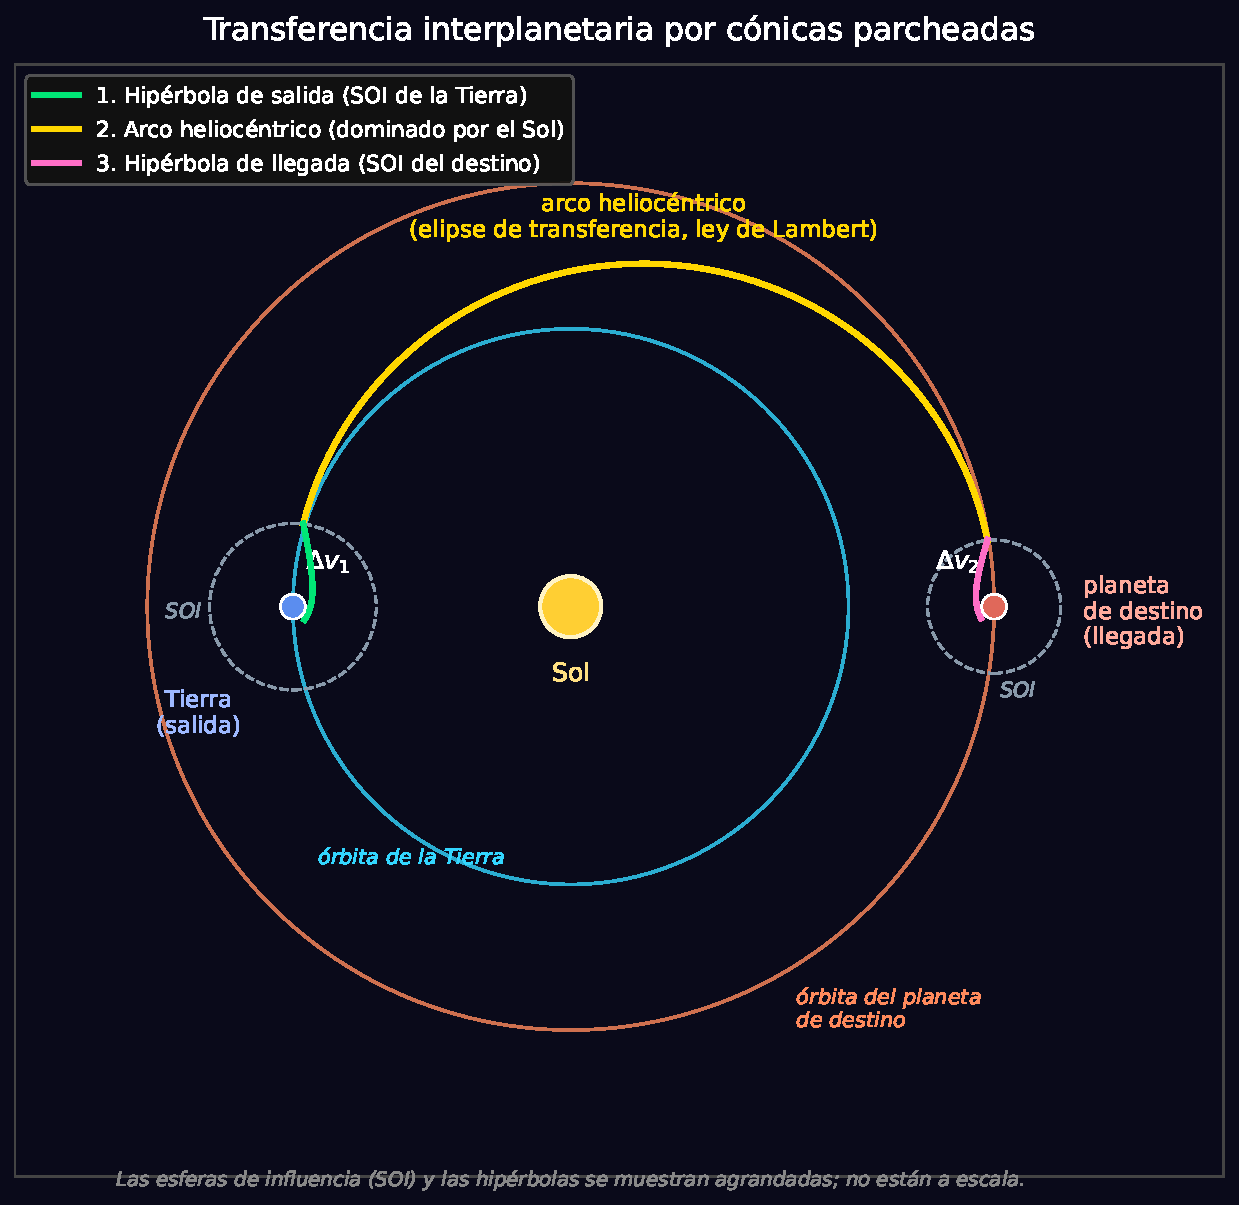
\includegraphics[width=0.86\textwidth]{tex/imagenes/fig_conicas_parcheadas.pdf}
  \caption{Transferencia interplanetaria por cónicas parcheadas. Elaboración propia.}
  \label{fig:conicas}
\end{figure}

La frontera entre tramos es la \gls{SOI} de cada planeta: la región a su alrededor en la que su gravedad domina sobre la del Sol. Dentro de la \gls{SOI} de la Tierra el movimiento se trata como una hipérbola de escape (gobernada por $\mu_{\text{Tierra}}$); fuera de ella, el trayecto es un arco heliocéntrico (gobernado por $\mu_{\text{Sol}}$); y a la llegada se ingresa en la \gls{SOI} del destino con otra hipérbola. Como la \gls{SOI} es muy pequeña frente a la distancia interplanetaria, en la práctica cada cosido se aproxima como un cambio instantáneo de velocidad ---por eso, en la figura~\ref{fig:conicas}, \gls{SOI} y las hipérbolas se dibujan agrandadas para poder apreciarlas---.

Esta aproximación es la que permite calcular el coste de la transferencia con las herramientas que siguen: el arco heliocéntrico se obtiene resolviendo el problema de Lambert, y los impulsos de salida y de llegada ---y la energía característica $C_3$--- resultan de comparar la velocidad de ese arco con la del planeta correspondiente.

\subsection{El problema de Lambert}
\label{sec:lambert}

El problema de Lambert consiste en hallar la órbita que une dos posiciones dadas, $\vec{r}_1$ y $\vec{r}_2$, en un tiempo de vuelo prefijado $\Delta t$ (Figura~\ref{fig:lambert}). Constituye, por tanto, un problema de contorno del movimiento de dos cuerpos: a diferencia de la propagación kepleriana ---que parte de una posición y una velocidad iniciales e integra la trayectoria hacia el futuro---, aquí se fijan los dos extremos de la trayectoria y la incógnita es la órbita que los enlaza en el tiempo dado. El problema no tiene solución analítica cerrada y se resuelve de forma iterativa.

Su resolución devuelve las dos velocidades sobre la órbita de transferencia: la velocidad necesaria en la salida, $\vec{v}_1$, y la de llegada, $\vec{v}_2$. El coste de la maniobra se obtiene comparándolas con las velocidades de los planetas en esos instantes (Ecuación \ref{eq:lambert-dv}):
\begin{equation}
  \Delta v_1 = \lvert \vec{v}_1 - \vec{v}_{\text{salida}} \rvert,
  \qquad
  \Delta v_2 = \lvert \vec{v}_{\text{llegada}} - \vec{v}_2 \rvert,
  \label{eq:lambert-dv}
\end{equation}
esto es, el impulso de inyección que abandona la órbita del planeta de partida y el de captura en el de destino. Esta es la base del diseño de transferencias interplanetarias y de los encuentros (\textit{rendezvous})\footnote{Maniobra en la que una nave debe coincidir con un objetivo móvil ---por ejemplo, para acoplarse a una estación---, ajustando no solo la órbita, sino también el instante de llegada.}.

\begin{figure}[htbp]
  \centering
  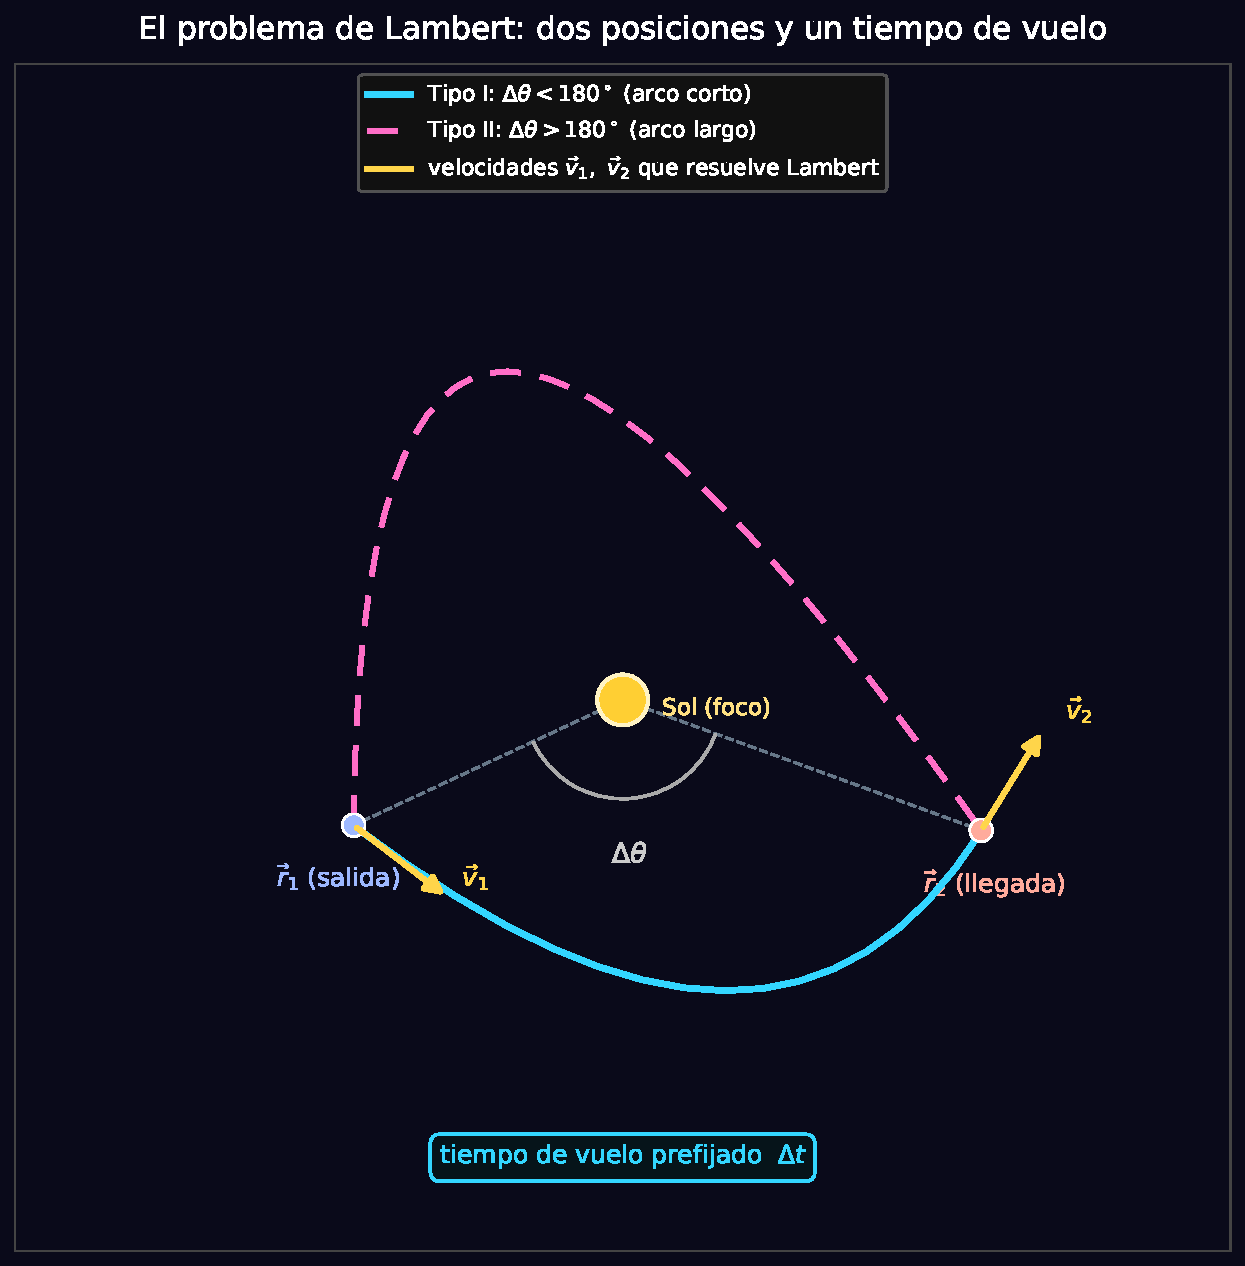
\includegraphics[width=0.78\textwidth]{tex/imagenes/fig_lambert.pdf}
  \caption{El problema de Lambert: dos posiciones y un tiempo de vuelo determinan la órbita de transferencia. Elaboración propia.}
  \label{fig:lambert}
\end{figure}

Para un par de posiciones y un tiempo de vuelo dados existen además dos familias de solución según el arco recorrido: las de \textbf{tipo~I} (ángulo de transferencia menor de $180^\circ$) y las de \textbf{tipo~II} (mayor de $180^\circ$). Ambas quedan separadas por la singularidad de los $180^\circ$, que se manifiesta como la franja diagonal del diagrama \textit{porkchop} (Figura~\ref{fig:porkchop}).

\subsection{Diagramas \textit{porkchop}}
\label{sec:porkchop}

Para una transferencia interplanetaria, el coste depende de cuándo se sale y cuándo se llega. Un diagrama \textit{porkchop} representa, mediante curvas de nivel, el coste ($\Delta v$ o la energía característica $C_3$, el cuadrado de la velocidad de exceso hiperbólico respecto al planeta de salida\footnote{La energía característica se define como $C_3 = v_\infty^2$, donde $v_\infty$ es la velocidad de exceso hiperbólico: la velocidad que conserva la nave una vez alejada del planeta de salida, ya fuera de su influencia gravitatoria. Tiene unidades de energía por unidad de masa ($\mathrm{km^2/s^2}$). Vale cero cuando la nave parte justo con la velocidad de escape (trayectoria parabólica) y es positiva para las trayectorias hiperbólicas, creciendo con la exigencia del viaje. Al depender únicamente de la trayectoria, y no del vehículo, se emplea como medida estándar para comparar el coste de lanzamiento entre misiones y la capacidad de carga de los lanzadores.}) en función de las fechas de salida y de llegada, y permite identificar las ventanas de lanzamiento óptimas. Estos diagramas se resuelven encadenando muchos problemas de Lambert. (Figura~\ref{fig:porkchop}). En el diagrama, cada punto es el coste $\Delta v$ de una transferencia según su fecha de salida (eje horizontal) y su tiempo de vuelo (eje vertical); las zonas amarillas son las más económicas y la estrella marca el óptimo (unos $5{,}78$~km/s para la ventana de 2026). La franja blanca diagonal corresponde a la singularidad de Lambert a $180^\circ$, que separa las soluciones de tipo~I y tipo~II.

\begin{figure}[htbp]
  \centering
  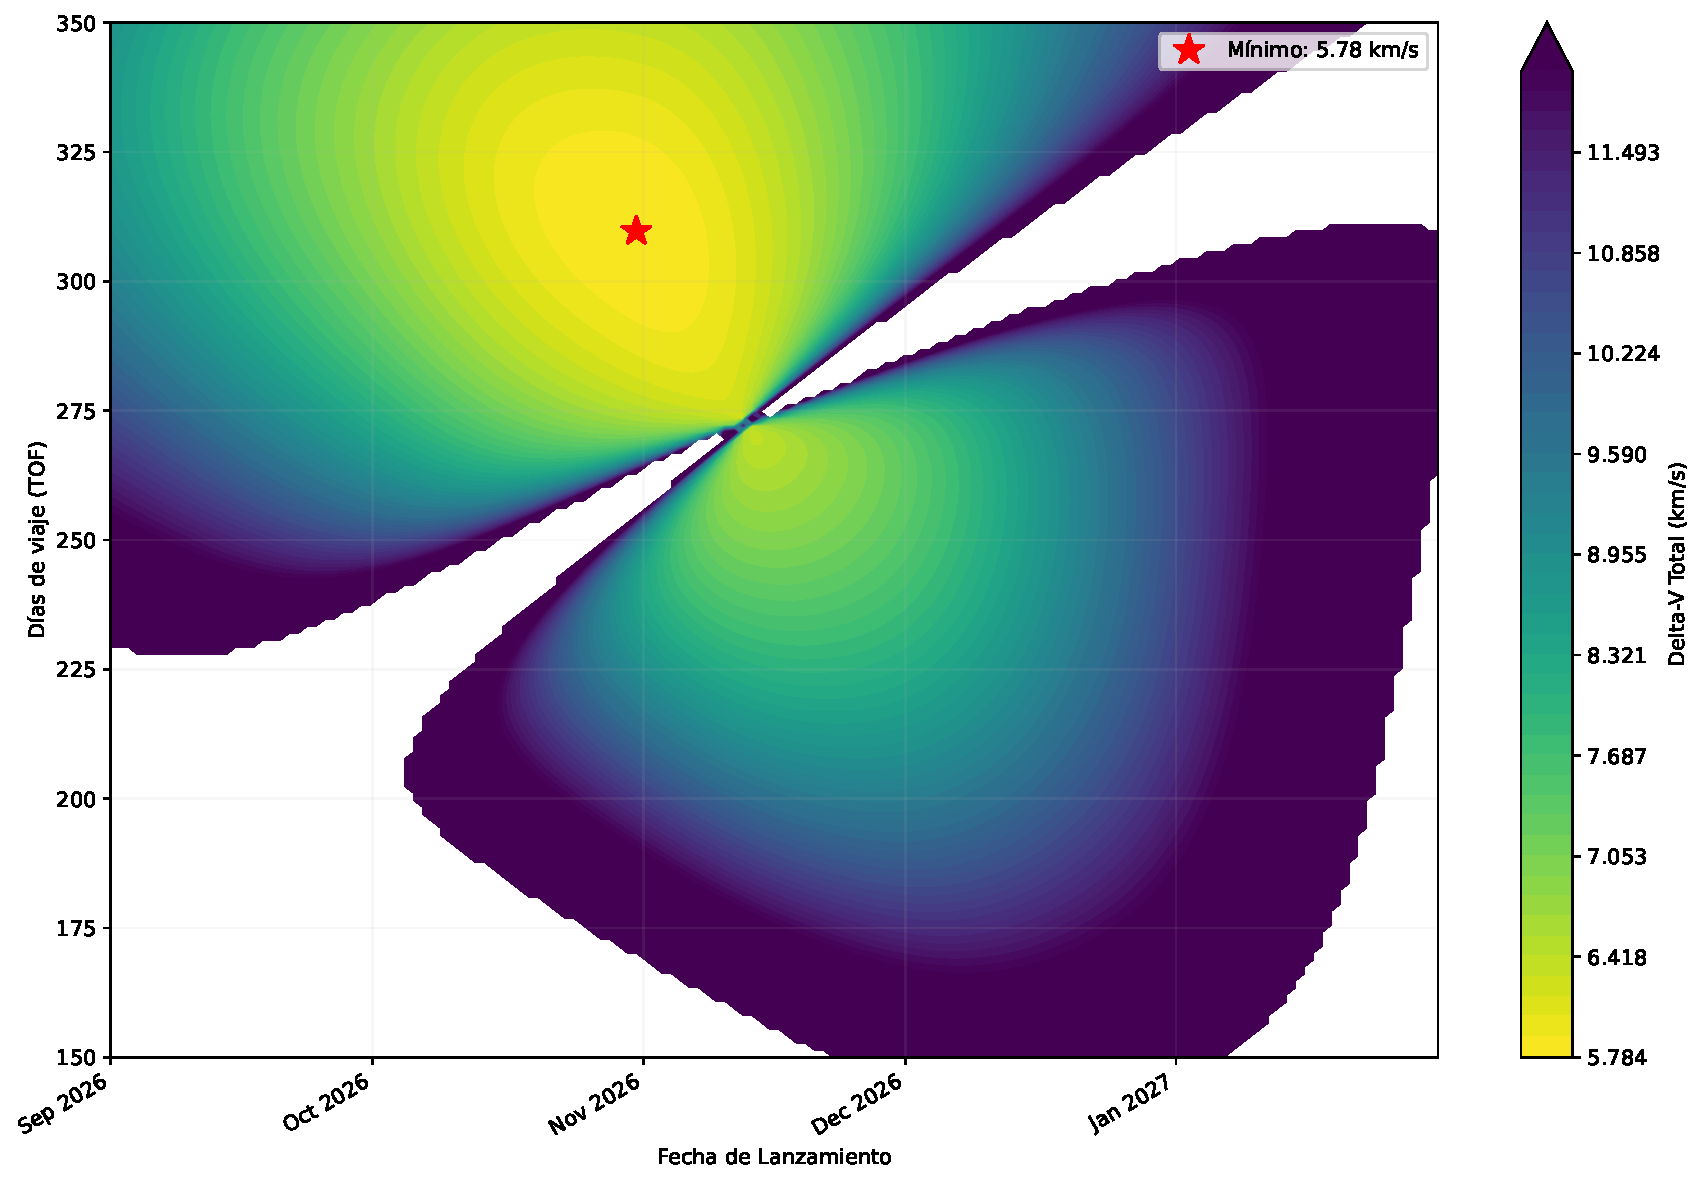
\includegraphics[width=0.9\textwidth]{tex/imagenes/porkchop_marte.pdf}
  \caption{Diagrama \textit{porkchop} de la transferencia Tierra--Marte para la ventana de 2026. Elaboración propia.}
  \label{fig:porkchop}
\end{figure}